\documentclass{beamer}
 
\usetheme{Madrid}
\usepackage{dirtytalk}
\usepackage{graphicx}
\graphicspath{ {./images/} }

\title{Predicting  A Personality Trait Using A Machine Learning Algorithm}
\subtitle{Senior Capstone I IT451 - 01}
\date{Spring 2020 4/22/20}
\author{Dustin Powell}
\institute{Cumberland University}

\begin{document}

\newtheorem{q1}{Primary Question}

 
\frame{\titlepage}

\begin{frame}
\frametitle{Table of Contents}
\begin{enumerate}
\item Introduction
\item PNAS Case Study
\item Analytics
\item Regression
\item Machine Learning
\item Experimental Planning
\item Experimental Setup
\item Experimental Results
\item Conclusion
\item References
\item Appendix
\end{enumerate}

\end{frame}

 %------------------------------------------------------------------------------
\begin{frame}
\frametitle{Introduction}
\footnotesize
\begin{itemize}
    \item According to Our World In Data, 3.5 billion people use the internet, with  2.3 billion using the social network Facebook\textsuperscript{\textregistered} \cite{IntStats}.
    \item About 640,000 new people access the internet daily \cite{IntStats}.
    \item More of people's \say{information} is becoming publicly viewable compared to before the creation of the internet.
    \item The purpose of this work is to use online data to demonstrate that using a limited amount of information can lead to uncovering private details about an individual. 
    \item A article published by the  Proceedings of the National Academy of Sciences of the United States of America (PNAS) demonstrates this predictability with statistics \cite{Kosinski2013}.
    \item Python code is used to further investigate the overall concept from the PNAS study.
\end{itemize}
\end{frame}

 %------------------------------------------------------------------------------
\begin{frame}
\frametitle{Case Study in PNAS}
\footnotesize
\begin{itemize}
    \item The post--liking habits of 58,466 people were able to predict various private aspects about the user, such as age, race, intelligence, and political views \cite{Kosinski2013}.
    \item The data collected had a overall average of  170 likes per user \cite{Kosinski2013}.
    \begin{figure}[ht]
\centering
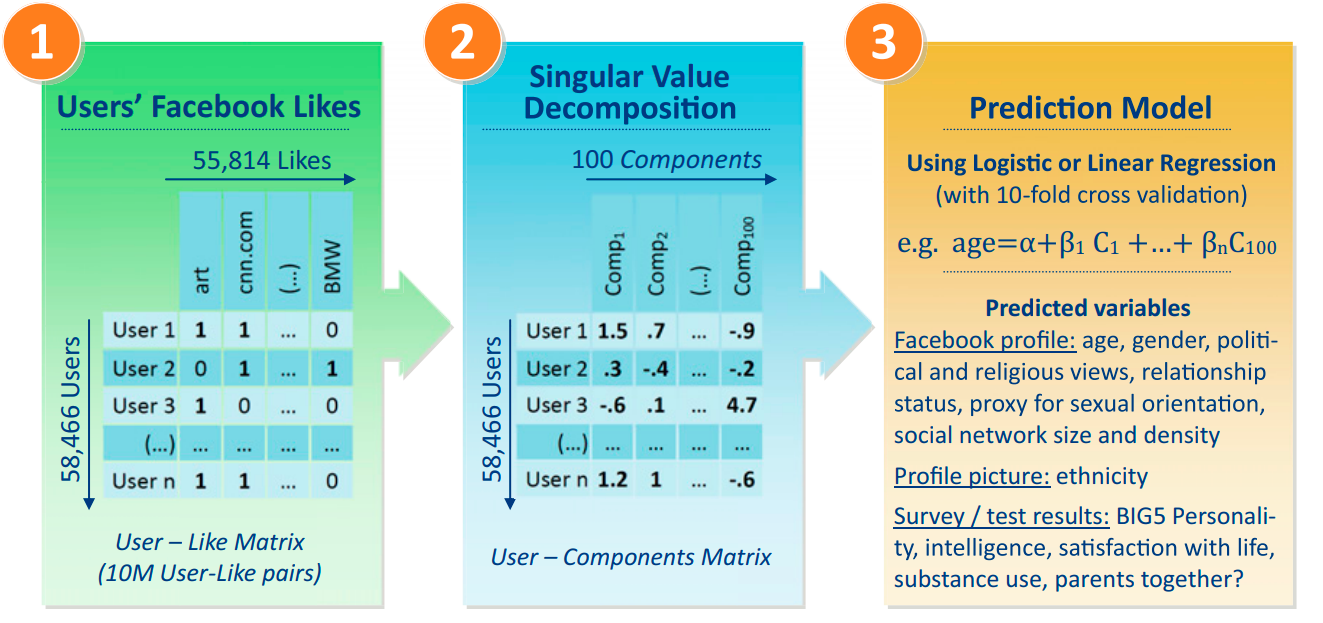
\includegraphics[scale=0.15]{PNAS}
\caption{ \footnotesize The process from the papers of the PNAS study outlining the steps used to make predictions with Facebook\textsuperscript{\textregistered} data \cite{Kosinski2013}.}
\end{figure}

\end{itemize}
\end{frame}

%------------------------------------------------------------------------------
\begin{frame}
\frametitle{Questions to Address}
\footnotesize
The alarming and possible harmful implications of the PNAS study prompts the following question.

\begin{q1}
Using a machine--learning algorithm what is the minimum amount of information needed to predict the personality trait of a given person accurately?
\end{q1}
Hypothesis:
\begin{enumerate}

\item A given person's personality trait is predictable with one feature.
\item An overall average accuracy score of 90 percent or higher can be obtained.
\item The overall average accuracy will increase as features in the model increase.
\end{enumerate}
\end{frame}

\begin{frame}
\frametitle{Big Data}
\footnotesize
 The case study conducted by Kosinski, Stillwell, and Gaepel (2013) reflects an overarching concept of a bigger project at hand called \textbf{big data}.
\newline
\newline
\textbf{Big Data} -- The mass collection of  data for the purpose of research by scientist,  government officials, and commercial institutions.
   \begin{itemize}
    \item Data is generated from users by visiting websites, liking posts, and watching videos get stored into large databases \cite{Jeble2016}. 

    \item The database are located in warehouses full of computers called servers that have a range of purposes \cite{Jeble2016}.

   \item Companies such as Google\textsuperscript{\textregistered}, Amazon\textsuperscript{\textregistered}, and Facebook\textsuperscript{\textregistered}
use these massive amounts of data to make predictions about their users \cite{Jeble2016}.
    \end{itemize}

\end{frame}

%------------------------------------------------------------------------------
\begin{frame}
\frametitle{Three Types of Data}
\footnotesize
Three types of data that are collected:
    \begin{itemize}
    \item \textbf{Structured} -- Any data that is clearly understood, defined, and can immediately store in databases without any preprocessing \cite{Jeble2016}.
        \begin{itemize}
        \item Example: Sales Figures
        \end{itemize}
    \item \textbf{Unstructured} -- Any data that is vague and convoluted, which requires the information to be further processed and organized for it to be of use and stored \cite{Jeble2016}.
        \begin{itemize}
        \item Example: Social Media Posts
        \end{itemize}
    \item \textbf{Semi--Structured} -- Any data considered the middle ground between structured and unstructured data and has some organized and unorganized aspects to the structure of the information \cite{Jeble2016}.
        \begin{itemize}
        \item Example: SQL Scripts, Server Logs
        \end{itemize}
    \end{itemize}

\end{frame}

%------------------------------------------------------------------------------
\begin{frame}
\frametitle{Forms of Analytics}

Three forms of analytics are performed on the data stored in databases \cite{Jeble2016}.
\begin{itemize}

    \item \textbf{Descriptive Analytics} -- Analysis of data from past occurrences of events.

    \item \textbf{Predictive Analytics} -- Analysis of data to make predictions.
    \item \textbf{Prescriptive Analytics} -- Analysis of data to make decisions.

\end{itemize}


\end{frame}

\begin{frame}
\frametitle{The Uses of Analytics}

The application of statistics and computer science allow for these various forms of analytics to be conducted and used in various ways \cite{Jeble2016}.

\begin{itemize}
    \item Analytics is used by businesses to make educated decisions by using the resource as a way to understand markets \cite{Jeble2016}.
    \item Predictive analytics can be used for predicting sales outcomes of a company's product versus the market competition \cite{Jeble2016}.
    \item Marketing uses predictive analytics to determine which advertisments to deliver to internet users \cite{Jeble2016}.
        \begin{itemize}
        \item Example: Youtube Video Advertisements 
        \end{itemize}
\end{itemize}
\end{frame}

%------------------------------------------------------------------------------
\begin{frame}
\frametitle{Overview of The Relationship}
\begin{figure}
\centering
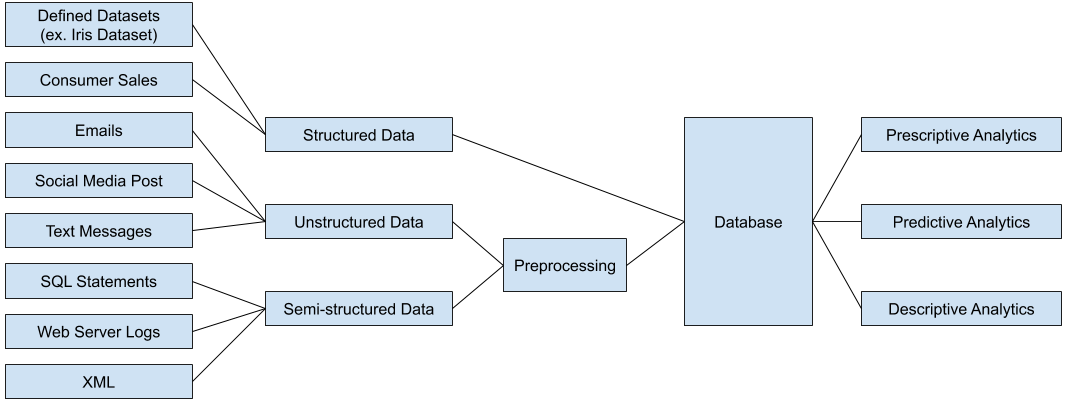
\includegraphics[scale=0.32]{Analytics}
\caption{\footnotesize The relationship between the three types of Big Data and analytics inspired, from the article by S. Jeble, S. Kumari, and Y. Patil \cite{Jeble2016}.}
\end{figure}
\end{frame}


%------------------------------------------------------------------------------
\begin{frame}
\frametitle{Regression and Predictive Analytics}
\scriptsize
One of the biggest purposes of collecting data is to find relationships that occur between data.
\newline
\newline
\textbf{Linear Regression}
\begin{itemize}
    \item Determines the possible correlation between two variables, one independent and one dependent using a function that best represents the correlation between the two variables with the smallest error between the correlation, $\hat{y}=\alpha+\beta X$ \cite{Stats2015}.
\end{itemize}
\begin{figure}[h]
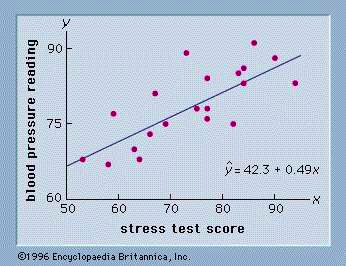
\includegraphics[scale=0.37]{LinReg}
\caption{ \scriptsize The correlation between blood pressure readings and stress test scores data. The x-axis represents stress test scores and the y-axis is blood pressure reading \cite{LinPNG}.}
\end{figure}

\end{frame}


%------------------------------------------------------------------------------
\begin{frame}
\frametitle{Regression and Predictive Analytic Continued}
\scriptsize
\textbf{Multiple Regression}
\begin{itemize}
    \item Determines the possible correlation between multiple independent and one dependent variables using a function that best represents the correlation \cite{Stats2015}.
\end{itemize}

\begin{figure}[h]
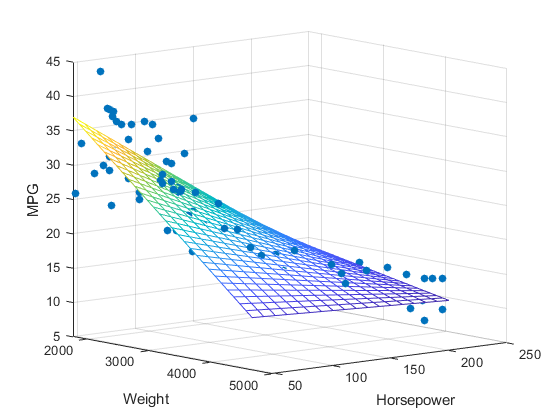
\includegraphics[scale=0.3]{MultiReg}
\caption{ \scriptsize Multiple regression plane created from a set of data containing miles per gallon of fuel, vehicle weight, and horsepower \cite{MultiPNG}.}
\end{figure}


\end{frame}

%------------------------------------------------------------------------------
\begin{frame}
\frametitle{What is Machine Learning}
\footnotesize
Machine Learning is a subsection of artificial intelligence that is specifically focused on using algorithms to make conclusions about a set of information \cite{pythonML}.
\newline
\newline
Their are three types of machine learning:
\begin{itemize}
 \item \textbf{Supervised Machine Learning} -- Using a base set of data to train the algorithm which then makes predictions based on the learned information \cite{pythonML}.
\item \textbf{Unsupervised Machine Learning} -- The use of an algorithm to classify and find relationships within a set of data without knowing of any results \cite{pythonML}.
\item \textbf{Reinforcement Machine Learning}
 -- The use of a agent that learns from task carried out that results in a reward for correctly carrying out the task \cite{pythonML}. \end{itemize}

\end{frame}

%------------------------------------------------------------------------------
\begin{frame}
\frametitle{The Iris Flower Data Set and Machine Learning}
\footnotesize
One of the most well--known data sets used for machine learning examples is the iris flower data set.
\newline
\begin{itemize}
    \item The iris data set consists of measurements were the sepal length and width, the petal length and width, and the subspecies name of each of the iris flowers \cite{pythonML}.
    \item Each flower within the data set can be known as an instance, object, or set of features \cite{pythonML}.
    \item The measurements that make up the flower are known as features \cite{pythonML}.
    \item The subspecies names of the flowers are called the class label or targets, which is the value to be predicted \cite{pythonML}. 
\end{itemize}

\begin{figure}[h]
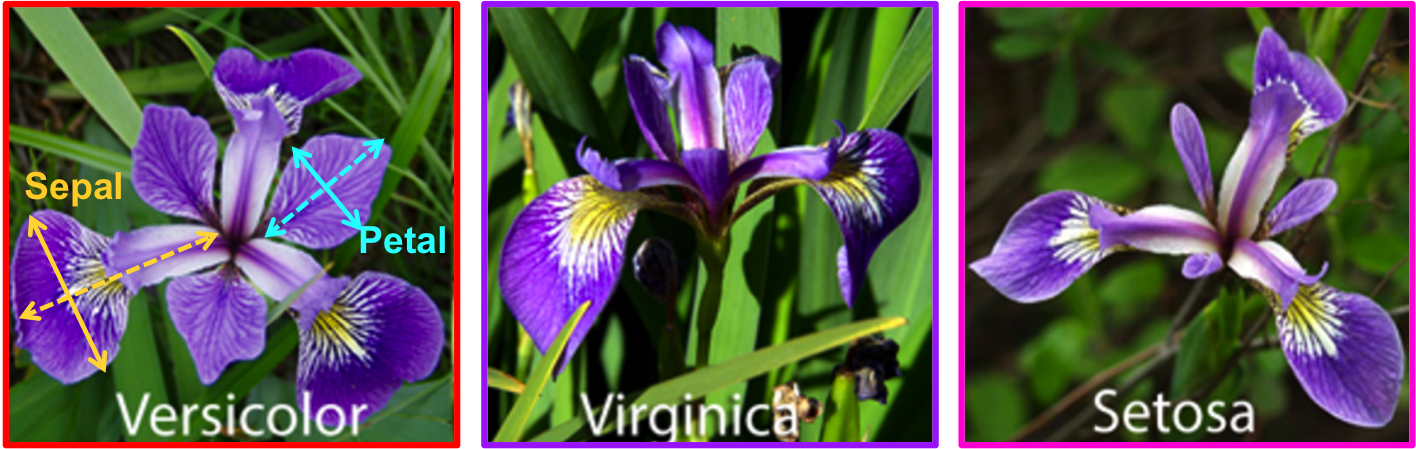
\includegraphics[scale=0.3]{iris}
\caption{ \scriptsize An image showing the iris flowers species and how they are measured \cite{IrisPNG}.}
\end{figure}

\end{frame}

%------------------------------------------------------------------------------
\begin{frame}
\frametitle{Internal Workings of Machine Learning (Artificial Neurons)}
\scriptsize
Machine learning makes decisions using artificial neurons \cite{pythonML}.
\begin{itemize}
    \item  \textbf{Artificial neuron} -- A mathematical representation of the neurons found in a biological brain \cite{pythonML}.
    \item Their are two types of neurons called the \textbf{perceptron} and \textbf{Adaline} \cite{pythonML}.
\end{itemize}
\begin{figure}[h]
\centering
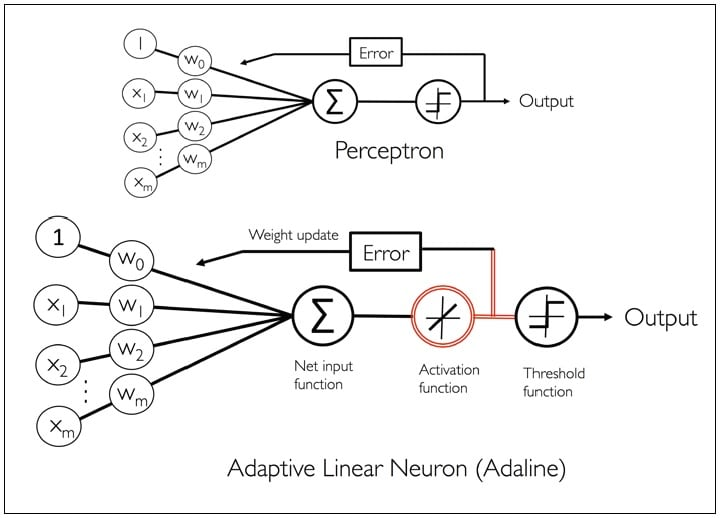
\includegraphics[scale=0.24]{neurons}
\caption{ \scriptsize A diagram that shows the structure of the perceptron and Adaline neurons \cite{Neuron}.}
\end{figure}
\end{frame}

%------------------------------------------------------------------------------
\begin{frame}
\frametitle{Internal Workings of Machine Learning (Artificial Neurons)}
\footnotesize
\textbf{Internal Workings of Machine Learning (Artificial Neurons)}
\newline

 Additionally, to further enhance the accuracy of the artificial neuron, multiple iterations over a set of data can be used to keep updating the weights to create an accurate model; with each of these times, the set of data goes through the artificial neuron is called an epoch \cite{pythonML}.
\newline
\newline
After an epoch, the weights update using the various functions depending on the type of artificial neuron used \cite{pythonML}. 
\newline
\newline
Just like the human brain, all of the artificial neurons can have connections to other artificial neurons creating a structure that resembles a human brain, which is called an \textbf{ artificial neural network} \cite{pythonML}.

\end{frame}

%------------------------------------------------------------------------------
\begin{frame}
\frametitle{Internal Workings of Machine Learning (Neural Network)}
\footnotesize
Three types of layers exist within a artificial neural network \cite{pythonML}.

\begin{itemize}
\item \textbf{Input Layer} -- The first set of neurons that interact with the data \cite{pythonML}.
\item \textbf{Output Layer} -- The layer that outputs the results concluded from the input data \cite{pythonML}.
\item \textbf{Hidden Layer} -- The layers between the input and output layer \cite{pythonML}.
\end{itemize}

A artificial neural network that contains multiple hidden layers is called a deep artificial neural network \cite{pythonML}.
\newline

One example of an artificial neural network is the multilayer perceptron (MLP)
\begin{itemize}
\item \textbf{Feedforward neural network} -- the artificial neurons' outputs as inputs for the next layer of artificial neurons \cite{pythonML}. 
\end{itemize}


\end{frame}


%------------------------------------------------------------------------------
\begin{frame}
\frametitle{Internal Workings of Machine Learning (Neural Network) Continued}
\scriptsize 
\begin{figure}[h]
\centering
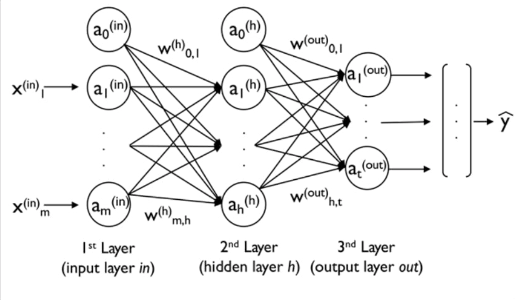
\includegraphics[scale=0.25]{NN}
\caption{ \scriptsize A diagram showing the layout of an artificial neural network called the mutilayer perceptron \cite{pythonML}.}
\end{figure}

The MLP has to conduct four necessary steps during each epoch to create an accurate model \cite{pythonML}. 
\begin{enumerate}
    \item Feed forward --  The data is sent through the neural network to determine an output \cite{pythonML}.
    \item Output is determined and the error is found by minimizing the utilization of a cost function \cite{pythonML}.
    \item Backpropgration -- Finding the derivative of the error using each weight in the model and updating the weights of the model repeats steps one through three as desired (epoch) \cite{pythonML}.
    \item Lastly, make predictions using forward propagation and a threshold function to predict an outcome \cite{pythonML}.
\newline
\end{enumerate}
\end{frame}

%------------------------------------------------------------------------------
\begin{frame}
\frametitle{Sub-types of Machine Learning}
\footnotesize
Sub-types of machine learning are:
\begin{itemize}
\item \textbf{Classification} -- A form of machine learning algorithms used to predict an output of one or more features from a set of input data \cite{pythonML}.
\item \textbf{Regression} -- Use of regression to make predictions from a set of data.
\item \textbf{Clustering} -- Group data together to find similarities between the elements in the dataset \cite{pythonML}.
\item \textbf{Dimensionality reduction} -- Shrinks the size of a set of data into smaller dimensions \cite{pythonML}. The primary use of dimensionality reduction is to create visualizations of complex graphs of a collection of data \cite{pythonML}. 
\end{itemize}

\end{frame}


%------------------------------------------------------------------------------
\begin{frame}
\frametitle{Sub-types of Machine Learning}

\begin{figure}[!h]
\centering
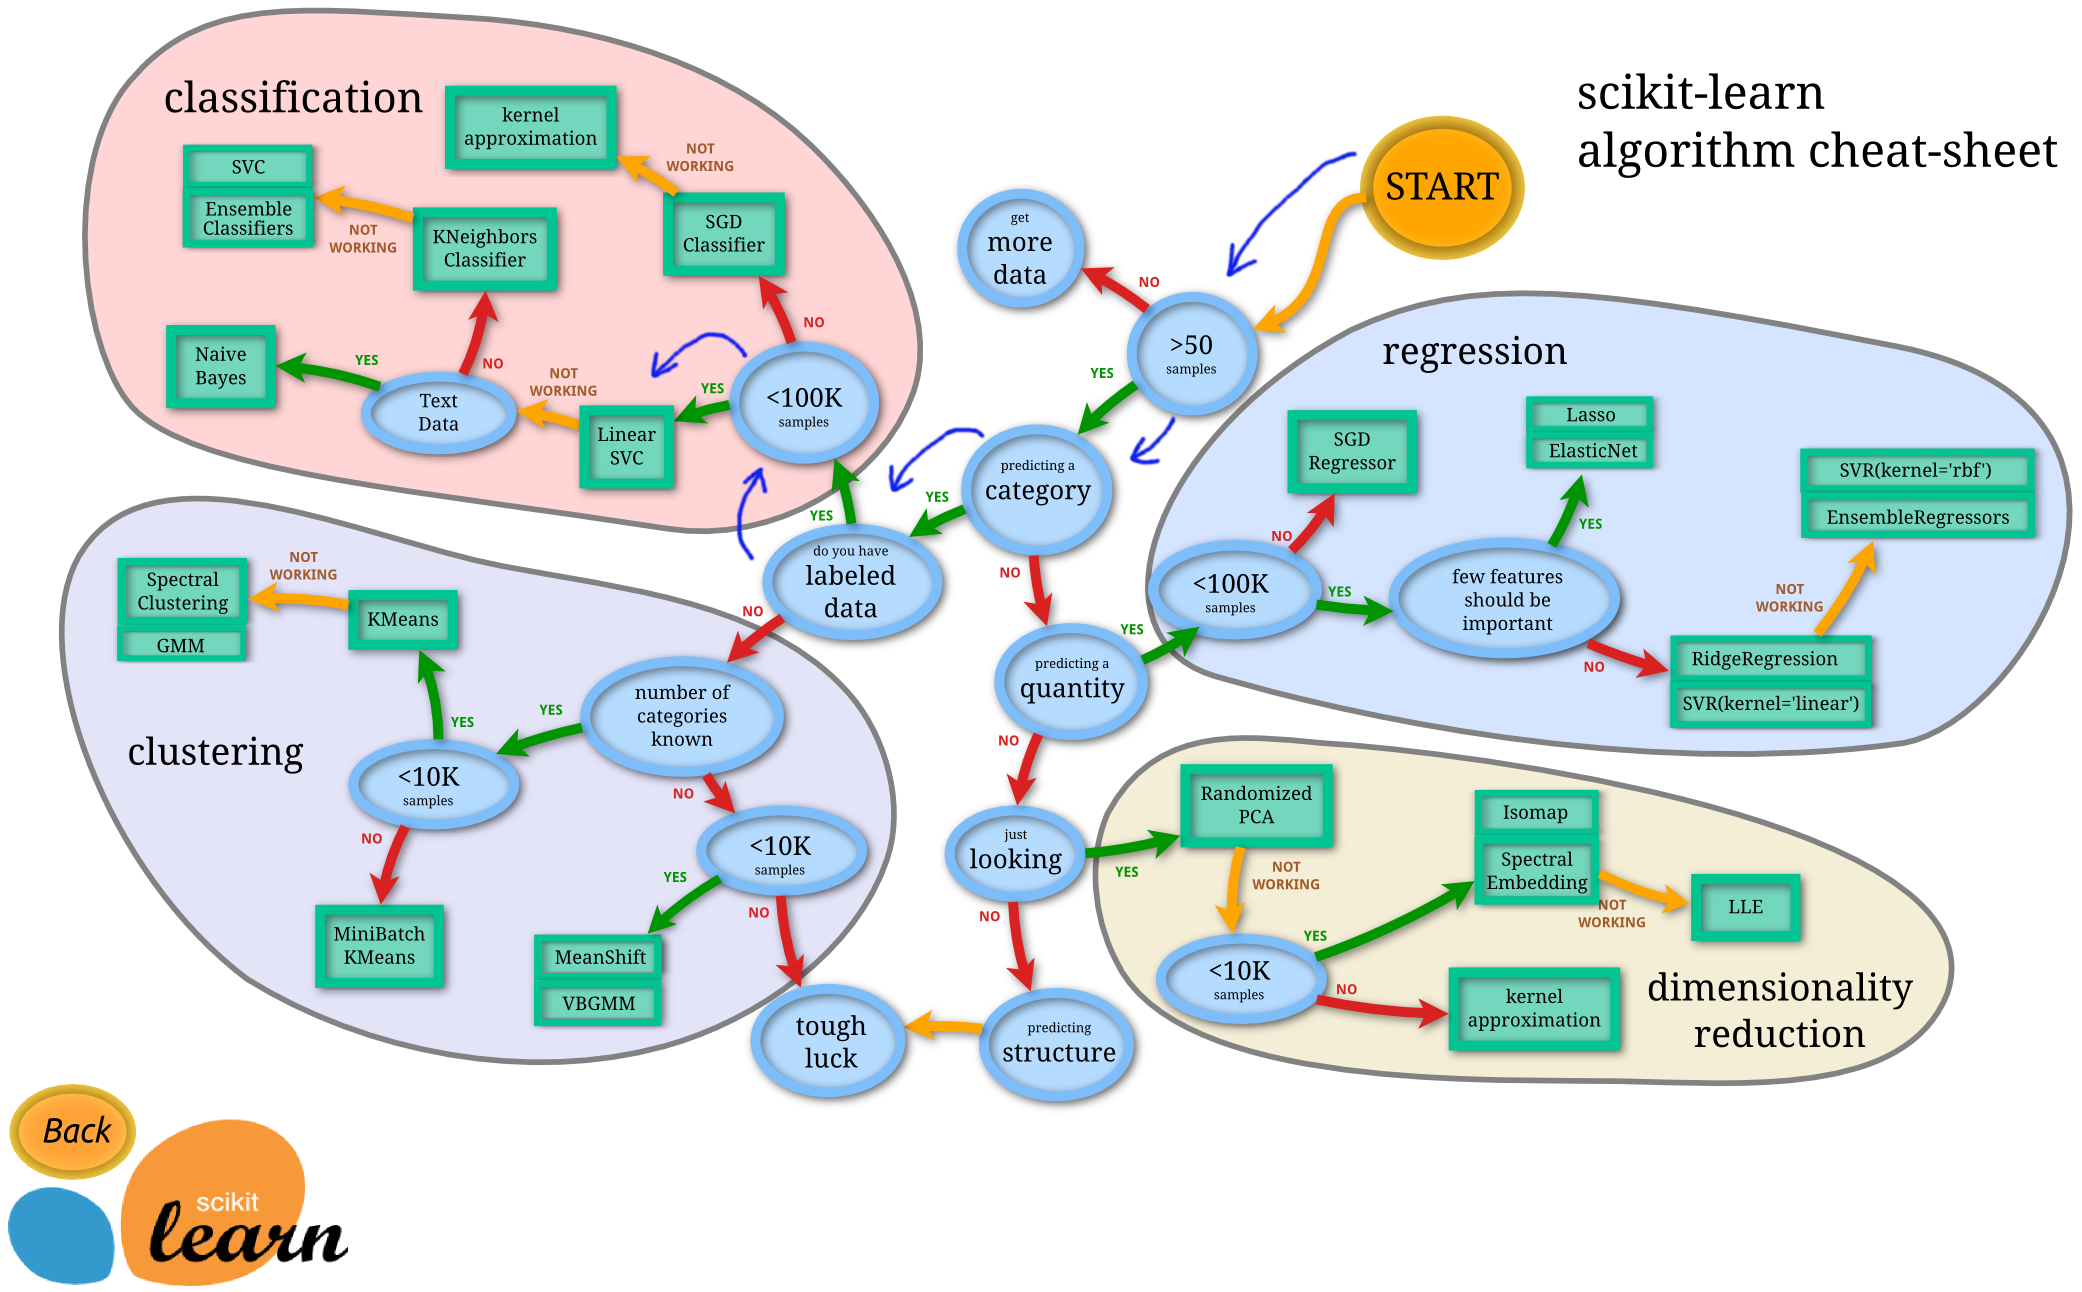
\includegraphics[scale=0.08]{ml_map}
\caption{ \footnotesize Map from the Scikit--learn website provided to help determine which estimators to use for machine learning \cite{SciKit}. The blue arrows represent the path taken. }
\end{figure}

\end{frame}

%------------------------------------------------------------------------------
\begin{frame}
\frametitle{Scikit--Learn Vs. TensorFlow}
\footnotesize
Two libraries and platforms used for machine learning with Python:
\newline

\textbf{Sci--kit Learn}
\begin{itemize}
\item Only uses Central Processing Unit (CPU) \cite{pythonML}.
\item Pre--made algorithms by various researchers \cite{SciKit}.
\item Can perform Classification, Regression, Clustering, and Dimensionality reduction \cite{SciKit}.
\end{itemize}

\textbf{TensorFlow}
\begin{itemize}
\item Can use CPU and graphics processing unit (GPU) for processing data \cite{pythonML}.
\item Has the same functions as Scikit--learn \cite{pythonML}.
\item Custom neural networks using tensors \cite{pythonML}.
\end{itemize}
 Sci--kit learn was chosen over to TensorFlow because of familiarity at an early stage of the project and time constraints of the project.
\end{frame}

%------------------------------------------------------------------------------
\begin{frame}
\frametitle{The Experiment's Plan}

Once a general understanding of the various topics was complete an experiment was set up in two parts.
\newline

\begin{enumerate}
\item A online data set.
\item An algorithm to process and display the information.
\end{enumerate}

The algorithm will have to be able to compare the results of the machine learning models using standardize variables to show the relationship between the amount of data the models are using to make predictions.

\end{frame}

%------------------------------------------------------------------------------
\begin{frame}
\frametitle{The Experiment's Plan Continued}

The standardized variables:
\newline

\begin{itemize}
\item Total time per set of models
\item Number of features analyzed by the models
\item Overall average accuracy score of analyzed models
\end{itemize}

One of the most important things about the algorithm is to make it easy to understand. The estimators and input data are designed to ensure that other parts in the code do not affect the final results of the test.

\end{frame}

%------------------------------------------------------------------------------
\begin{frame}
\frametitle{The Dataset}

The chosen dataset is a study posted on Kaggle.com of people between the ages 15 and 30 years old  with over 1000 responses \cite{DataSet}. 
\newline

The question within the survey pertained to music, movies, hobbies and interests, phobias, health habits, spending habits, and demographics \cite{DataSet}. 
\newline 
\newline 
The study contains 150 questions overall, with the majority over the topics of personality traits, views on life, and opinions \cite{DataSet}.
\newline
\newline
The most of the questions are recorded as integers 1 through 4, and others based on category phrases \cite{DataSet}.

\end{frame}

%------------------------------------------------------------------------------
\begin{frame}
\frametitle{The Dataset Preparation For Testing}
The data was manually preprocessed with LibreOffice Calc
\newline

\begin{enumerate} 
\item Phrases were changed to integer responses
\item Missing values were set to 999
\item The data was split into seven CSV files that had to match the set a features being tested
\end{enumerate}


The predicted question from the survey is anger with the output as the interger rating according to the survey. The features used to predict a person's anger are the spending habit questions.


\end{frame}

%------------------------------------------------------------------------------
\begin{frame}
\frametitle{The Project Algorithm}
\footnotesize

The Main Challenge
\begin{itemize}
\item Choosing the proper estimator to work with as there are many of them.
\end{itemize}


The diagram recommends using the algorithms SVM and KNearestNeighbor, but we ultimately decided to use Scikit--learn's version of the multilayer perceptron called the MLPClassifer, which is not listed on the diagram \cite{SciKit}.
\newline

The selection of the MLPClassifer ultimately leads up to the final algorithm after numerous instances of tinkering with the machine--learning code.
\newline

The code is divided into three sections called Data Handling, Model Creation and Prediction, and Displaying Results.
\newline

The code was inspired from a sample set by Jason Brownlee from machinelearningmastery.com that is used on the iris dataset \cite{MLMaster}.
\end{frame}

%------------------------------------------------------------------------------
\begin{frame}
\frametitle{The Project Algorithm}

The models follows the following step within the program algorithm.
\begin{enumerate}
\item Read Data -- Loading data from file.
\item Create Model -- Using estimator to make the model.
\item Validate Model -- Determine the accuracy of the model.
\item Store Results -- Calculates and stores the result for a set of models.
\item Repeat last three steps till all sets of features are analyzed with all estimators.
\item Display Collected Data -- Data stored is plotted on to 3D scatter plot for analysis. 
\end{enumerate}
\end{frame}

%------------------------------------------------------------------------------
\begin{frame}
\frametitle{The Experiment}

The experiment will have three tests with each of the three estimators creating models from the set of features each test. 
\newline

The number of models analyzed per set of features is set to ten.

\begin{itemize}
\item Estimator 1: Sci--kit learn default parameters with 1400 epochs.
\item Estimator 2: The activation function is configured to tangent with 1400 epochs.
\item Estimator 3: The activation function is set to logistic with 1400 epochs.
\end{itemize}
The reason the number of epochs are the same is because of convergence problems with the estimators were not reaching the most optimized point to determine the weights.

\end{frame}



%------------------------------------------------------------------------------
\begin{frame}
\frametitle{The Results: Test 1}
\begin{figure}
\centering
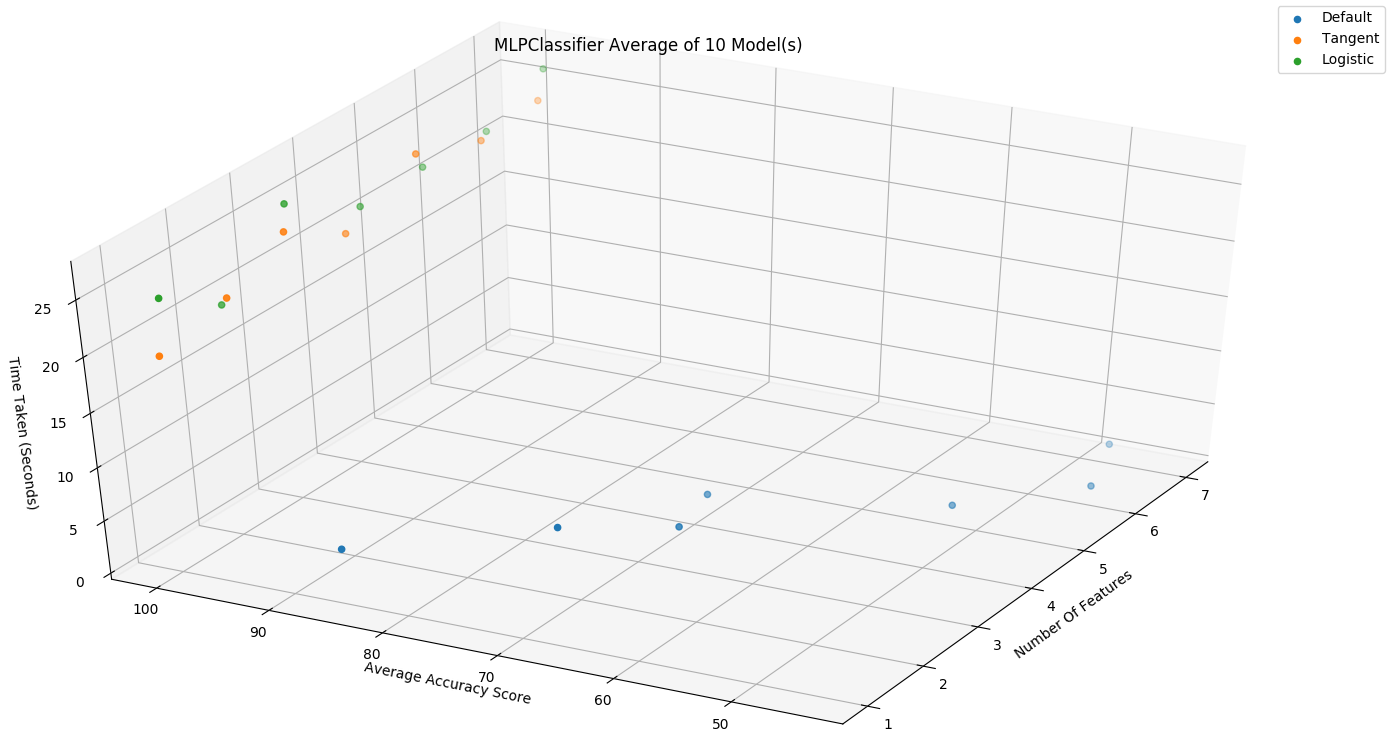
\includegraphics[scale=0.335]{Test_1}
\caption{\scriptsize The results of the first test results of the MLPClassifer Comparison algorithm. X--axis is Number of Features, Y--axis is average accuracy score, and Z--axis is Time Taken in seconds.}
\end{figure}
\end{frame}

%------------------------------------------------------------------------------
\begin{frame}
\frametitle{The Results: Test 2}
\begin{figure}
\centering
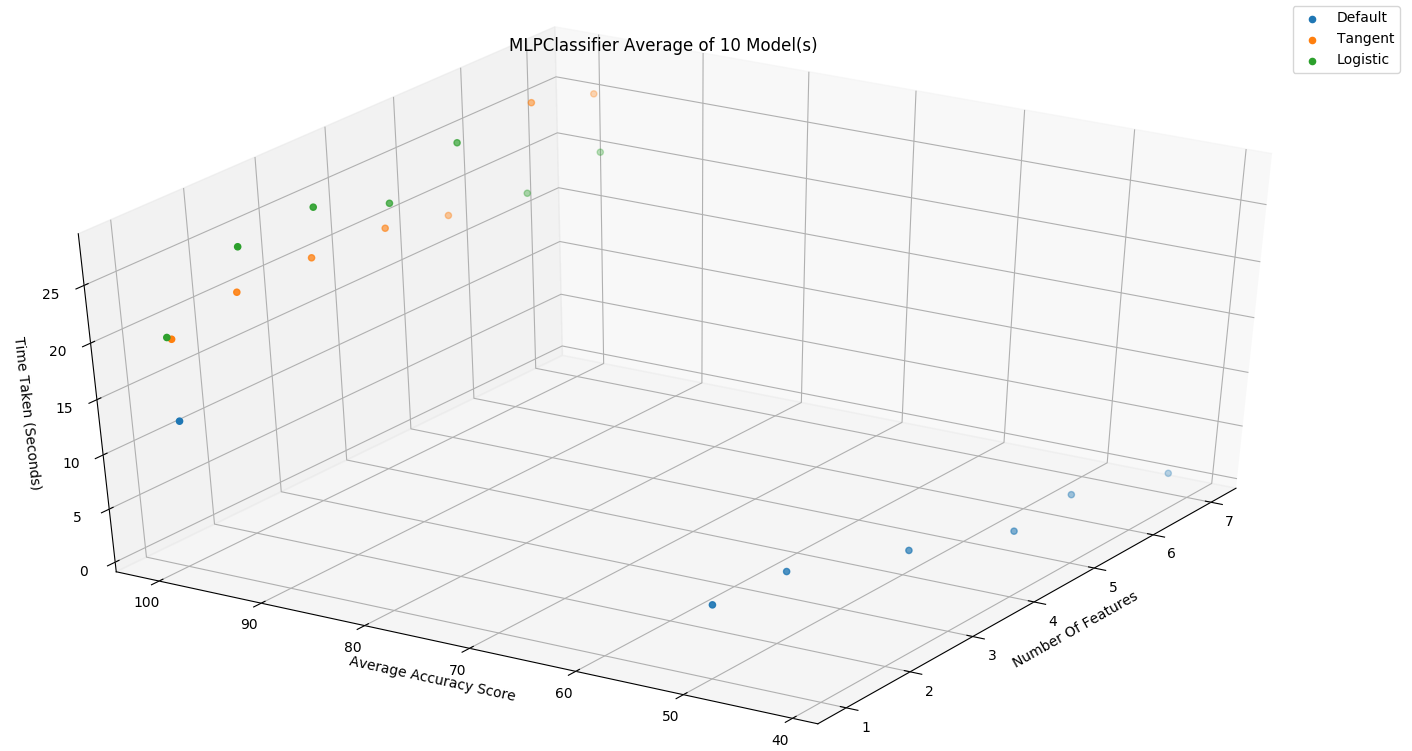
\includegraphics[scale=0.335]{Test_2}
\caption{\scriptsize The results of the second test results of the MLPClassifer Comparison algorithm. X--axis is Number of Features, Y--axis is average accuracy score, and Z--axis is Time Taken in seconds.}
\end{figure}
\end{frame}

%------------------------------------------------------------------------------
\begin{frame}
\frametitle{The Results: Test 3}
\begin{figure}[h]
\centering
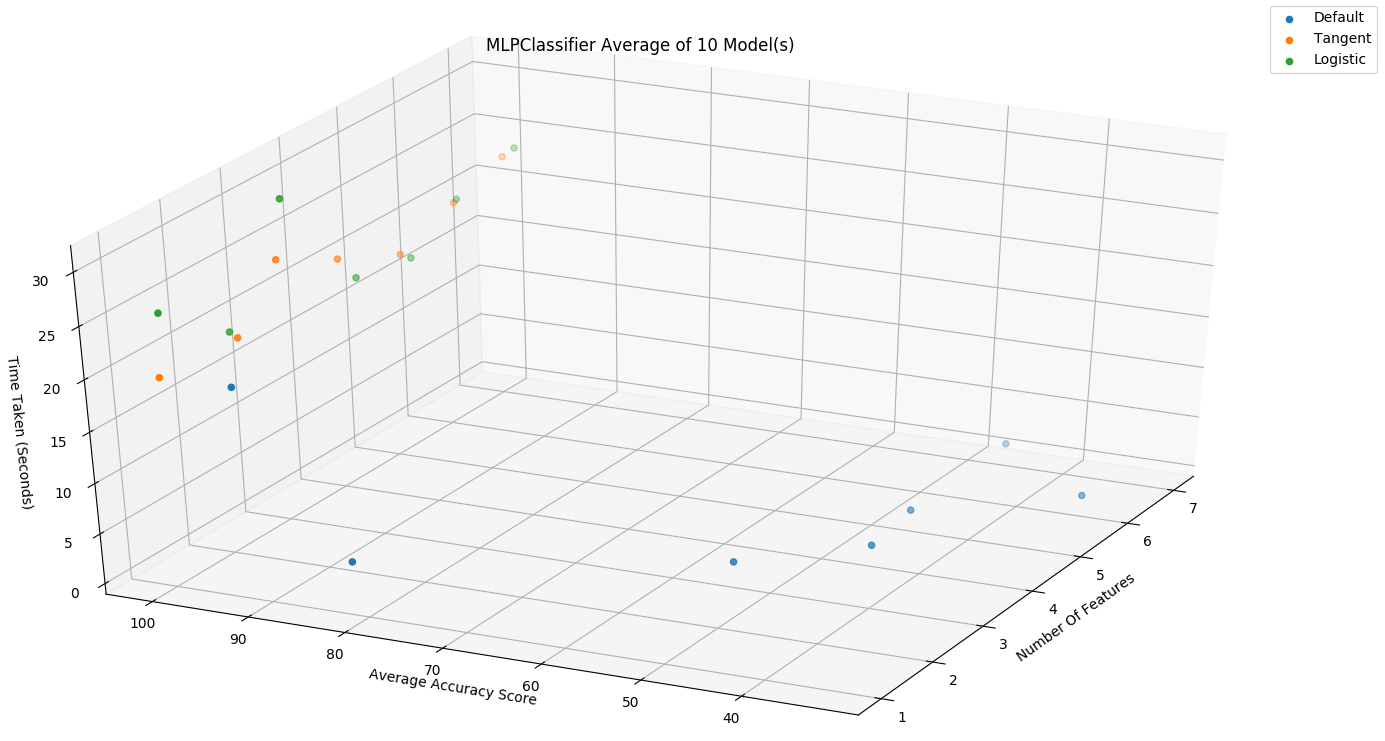
\includegraphics[scale=0.335]{Test_3}
\caption{\scriptsize The results of the third test results of the MLPClassifer Comparison algorithm. X--axis is Number of Features, Y--axis is average accuracy score, and Z--axis is Time Taken in seconds.}
\end{figure}
\end{frame}

%------------------------------------------------------------------------------
\begin{frame}
\frametitle{The Results: Conclusion}
\footnotesize
After the testing was complete it led to the following conclusions:
\begin{itemize}
\item Out of all three tests combined, the Tangent and Logistic models had a higher average accuracy score but took more time to create and validate. 
\item The Default models were sporadic, with the majority of the one feature average accuracy scores being above at least 80 percent.

\item The personality of a person with one feature is predictable using a multilayer perceptron classifier. 

\item The estimators must be tuned and tested to have the models make accurate predictions about a personality trait of a person.
\end{itemize}

\end{frame}


%------------------------------------------------------------------------------
\begin{frame}
\frametitle{Future Works}
\footnotesize
Given the results and concepts learned from the project, some other aspects could have been included.
\begin{itemize}
\item All parameters of the MLPClassifer could have been tested during the project, like the effects of tolerances on models.
\item More depth by observing every process of multiple machine learning algorithms in exquisite detail, outlining the many mathematical algorithms that enable machine learning to work.
\item Other types and sub-types of machine learning could have been used to investigate the data further and make conclusions from the data.
\end{itemize}
The overall limiting factor of the project is the time constraint of only one semester. 
\newline

The work can be further built upon to analyze the data set or continue learning about the topic of machine learning.

\end{frame}

%------------------------------------------------------------------------------
\begin{frame}
\frametitle{Conclusion}
\footnotesize
Key take--aways from the project:
\begin{itemize}
\item Only one feature is needed to predict the personality trait of a given person.
\item The goal was accomplished by fine-tuning of the parameters of the estimators to increase the accuracy score of the models.
\item The broadness of predictive analytics implies that many industries use analytics for different purposes but have a common ground.
\item Self--learning, self--discipline, and practice can allow for new exciting things to be learned.
\end{itemize}

\end{frame}


%------------------------------------------------------------------------------
\begin{frame}
\frametitle{References}
\tiny
\begin{thebibliography}{9}

\bibitem[1]{IntStats}
M. Roser, H. Ritchie, and E. Ortiz-Ospina (2020),
\say{Internet}. Published online at OurWorldInData.org. Retrieved from: 'https://ourworldindata.org/internet' [Website]

\bibitem[2]{Kosinski2013}
M. Kosinski, D. Stillwell, and T. Graepel (2013),
\say{Private traits and attributes are predicatable from digital records of human behavior}, \textit{PNAS} 110. 15. , 5802 - 5805. Google Scholar. Accessed January 19th 2020 URL: https://www.pnas.org/content/pnas/110/15/5802.full.pdf [Journal]

\bibitem[3]{Jeble2016}
S. Jeble, S. Kumari, and Y. Patil (2016),
\say{Role of big data and predictive analytics}. \textit{International Journal of Automation and Logistics}. 2. 307-331. 10.1504/IJAL.2016.10001272. Google Scholar. Accessed January 21st 2020 URL: https://www.researchgate.net/publication/309809606 [Journal]

\bibitem[4]{Stats2015}
J. Bothe, J. L. Brudney, and K. J. Meier (2015), 
\textit{Applied Statistics For Public and Nonprofit Administration}. 4th ed. Stamford, CT USA Cengage Learning. [eBook]

\bibitem[5]{pythonML}
V. Mirjalili and S. Raschka (2017),
\textit{Python Machine Learning}. 2nd ed. Birmingham, UK Packt Publishing. [eBook]

\bibitem[6]{IrisData}
\say{Iris Data Set'}, University of California Irvine Machine Learning Repository. Accessed February 5th 2020 URL: https://archive.ics.uci.edu/ml/datasets/iris [Website]

\bibitem[7]{DataSet}
M. Sabo (2016), \say{2013 Young People Survey}. Accessed February 13th 2020 URL: https://www.kaggle.com/miroslavsabo/young-people-survey [Website]

\end{thebibliography}
\end{frame}

\begin{frame}
\frametitle{References Continued}
\tiny
\begin{thebibliography}{9}

\bibitem[8]{SciKit}
\say{scikit-learn Machine Learning in Python}. Accessed February 17th 2020 URL: https://scikit-learn.org/stable/index.html [Website]

\bibitem[9]{Neuron}
www.simplilearn.com (n.d),
\say{How to Train an Artificial Neural Network}. Accessed April 13th 2020 URL: https://www.simplilearn.com/how-to-train-artificial-neural-network-tutorial [Online Image]

\bibitem[10]{PrinDS}
S. Kakade, S. Ozdemir, and M. Tibaldeschi (2018),
\textit{Principles of Data Science}. 2nd ed. Birmingham, UK Packt Publishing Ltd. [eBook]

\bibitem[11]{LinPNG}
D. Anderson, D. Sweeney, and T. Williams (2020),
\say{Statistics}, Encyclopaedia Britannica. Accessed March 23rd 2020 
URL: https://www.britannica.com/science/statistics/Experimental-design\#ref367488 [Online Image]

\bibitem[12]{MultiPNG}
\say{regress} (n.d), MathWorks. Accessed March 23rd 2020 URL: https://www.mathworks.com/help/stats/regress.html [Online Image]

\bibitem[13]{SVD}
J. Brownless (2018),
\say{How to Calculate the SVD from Scratch with Python}. Accessed March 30th 2020 URL: https://machinelearningmastery.com/singular-value-decomposition-for-machine-learning/ [Website]

\bibitem[14]{Cost}
K. Krzyk (2018),
\say{Coding Deep Learning for Beginners Linear Regression (Part 2): Cost Function}. Accessed March 30th 2020 URL: https://towardsdatascience.com/coding-deep-learning-for-beginners-linear-regression-part-2-cost-function-49545303d29f [Website]

\bibitem[15]{MLMaster}
J. Brownlee (2020),
\say{Your First Machine Learning Project in Python Step-By-Step}. Accessed February 5th 2020 URL: https://machinelearningmastery.com/machine-learning-in-python-step-by-step/ [Website]

\bibitem[16]{IrisPNG}
S. Flaloke (2016),
\say{Classification of Iris Varieties}. Accessed April 21st 2020 URL: http://suruchifialoke.com/2016-10-13-machine-learning-tutorial-iris-classification/ [Online Image]

 \end{thebibliography}
\end{frame}

%------------------------------------------------------------------------------
\begin{frame}
\frametitle{Thank You}
\Large
\center
\centering

Thank you for your time to attend the presentation.
\newline

Please do not hesitate to ask questions.
\newline

(By the way, if doing a senior project, start early.)
\end{frame}

%------------------------------------------------------------------------------
\begin{frame}[fragile]
\frametitle{The Project Code: Initialization}

\fontsize{6}{5}
The initialization of variables for the program.
\begin{verbatim}
#Main Function ----------------------------------------------------------------
def main():

    #Local Declarations -----------------------------------

    #Initialization of variables
    average = 10              #Number of times to make a model to determine
                              # overall average accuracy score

    feature = [1,2,3,4,5,6,7] #List of the amount of features used per model

    MLPdata1 = []             #List to store overall average accuracy
                              # of MLPClassifier

    MLPdata2 = []             #List to store overall average accuracy
                              # of MLPClassifier

    MLPdata3 = []             #List to store overall average accuracy
                              # of MLPClassifier

    final_time1 = []          #List to store time taken to analyze both models
                              # with n features

    final_time2 = []          #List to store time taken to analyze both models
                              # with n features

    final_time3 = []          #List to store time taken to analyze both models
                              # with n features

\end{verbatim}

\end{frame}

%-------------------------------------------------------------------------------

\begin{frame}[fragile]
\frametitle{The Project Code: Data Handling Section}

\fontsize{6}{5}
\begin{verbatim}
#Local Statements -------------------------------------

    #SECTION: Data Handling----------------------------------------------------

    print("        MLPClassifier Model Comparison         ")
    print("-----------------------------------------------")
    print("Please wait until the 3D scatter plot displays ")

    #For loop to iterate through all models being observed
    for iter_selection in range(3):
  
        #For loop to iterate through data sets used by the models and estimators
        for i in range(7):

            #If statements to that determine which set of data is being used
            if i == 0:
                #Load data set values from CSV file
                csvData = "responses-1feature-finances.csv"
                
                #Array to store names of feature(s) and target feature
                names = ['Getting angry', 'Finances']

                #Stores the data values with names of questions
                dataset = read_csv(csvData, names=names)

                #Stores array values into an array
                array = dataset.values

                #Initialization of two NumPy X and y arrays
                X1 = array[:,0:2]
                y1 = array[:,0]

                #Function to split the question values into a training set where 20 percent of the 
                # data set is used for validation
                (X_train, X_validation, Y_train, Y_validation) = train_test_split(X1, y1, test_size=0.20)
\end{verbatim}
\end{frame}

%-------------------------------------------------------------------------------


\begin{frame}[fragile]
\frametitle{The Project Code: Data Handling Section}

\fontsize{6}{5}
\begin{verbatim}
            if i == 1:
                #Load data set values from CSV file
                csvData = "responses-2features.csv"    

                #Array to store names of feature(s) and target feature
                names = ['Getting angry', 'Finances','Shopping centres']
    
                #Stores the data values with names of questions
                dataset = read_csv(csvData, names=names)

                #Stores array values into an array
                array = dataset.values

                #Initialization of two NumPy X and y arrays
                X2 = array[:,0:3]
                y2 = array[:,0]

                #Function to split the question values into a training set where 20 percent of the 
                # data set is used for validation
                (X_train, X_validation, Y_train, Y_validation) = train_test_split(X2, y2, test_size=0.20)

            if i == 2:
                #Load data set values from CSV file
                csvData = "responses-3features.csv"    

                #Array to store names of feature(s) and target feature
                names = ['Getting angry', 'Finances','Shopping centres', 'Branded clothing']
    
                #Stores the data values with names of questions
                dataset = read_csv(csvData, names=names)

                #Stores array values into an array
                array = dataset.values

                #Initialization of two numpy X and y arrays
                X3 = array[:,0:4]
                y3 = array[:,0]

                #Function to split the question values into a training set where 20 percent of the 
                # data set is used for validation
                (X_train, X_validation, Y_train, Y_validation) = train_test_split(X3, y3, test_size=0.20)


\end{verbatim}
\end{frame}

%-------------------------------------------------------------------------------

\begin{frame}[fragile]
\frametitle{The Project Code: Data Handling Section}

\fontsize{6}{5}
\begin{verbatim}
            if i == 3:
                #Load data set values from CSV file
                csvData = "responses-4features.csv"

                #Array to store names of feature(s) and target feature
                names = ['Getting angry', 'Finances','Shopping centres', 'Branded clothing',
                         'Entertainment spending']
    
                #Stores the data values with names of questions
                dataset = read_csv(csvData, names=names)

                #Stores array values into an array
                array = dataset.values

                #Initialization of two numpy X and y arrays
                X4 = array[:,0:5]
                y4 = array[:,0]

                #Function to split the question values into a training set where 20 percent of the 
                # data set is used for validation
                (X_train, X_validation, Y_train, Y_validation) = train_test_split(X4, y4, test_size=0.20)

\end{verbatim}
\end{frame}

%-------------------------------------------------------------------------------

\begin{frame}[fragile]
\frametitle{The Project Code: Data Handling Section}

\fontsize{6}{5}
\begin{verbatim}
            if i == 4:
                #Load data set values from CSV file
                csvData = "responses-5features.csv"    

                #Array to store names of feature(s) and target feature
                names = ['Getting angry', 'Finances','Shopping centres', 'Branded clothing',
                         'Entertainment spending', 'Spending on looks']
    
                #Stores the data values with names of questions
                dataset = read_csv(csvData, names=names)

                #Stores array values into an array
                array = dataset.values

                #Initialization of two numpy X and y arrays
                X5 = array[:,0:6]
                y5 = array[:,0]

                #Function to split the question values into a training set where 20 percent of the 
                # data set is used for validation
                (X_train, X_validation, Y_train, Y_validation) = train_test_split(X5, y5, test_size=0.20)

\end{verbatim}
\end{frame}


%-------------------------------------------------------------------------------

\begin{frame}[fragile]
\frametitle{The Project Code: Data Handling Section}

\fontsize{6}{5}
\begin{verbatim}
            if i == 5:
                #Load data set values from CSV file
                csvData = "responses-6features.csv"    

                #Array to store names of feature(s) and target feature
                names = ['Getting angry', 'Finances','Shopping centres', 'Branded clothing',
                        'Entertainment spending', 'Spending on looks', 'Spending on gadgets']
    
                #Stores the data values with names of questions
                dataset = read_csv(csvData, names=names)

                #Stores array values into an array
                array = dataset.values

                #Initialization of two numpy X and y arrays
                X6 = array[:,0:7]
                y6 = array[:,0]

                #Function to split the question values into a training set where 20 percent of the 
                # data set is used for validation
                (X_train, X_validation, Y_train, Y_validation) = train_test_split(X6, y6, test_size=0.20)
\end{verbatim}
\end{frame}

%-------------------------------------------------------------------------------

\begin{frame}[fragile]
\frametitle{The Project Code: Data Handling Section}

\fontsize{6}{5}
\begin{verbatim}

            if i == 6:
                #Load data set values from CSV file
                csvData = "responses-7features.csv"    

                #Array to store names of feature(s) and target feature
                names = ['Getting angry', 'Finances','Shopping centres', 'Branded clothing',
                         'Entertainment spending', 'Spending on looks', 'Spending on gadgets',
                         'Spending on healthy eating']
    
                #Stores the data values with names of questions
                dataset = read_csv(csvData, names=names)

                #Stores array values into an array
                array = dataset.values

                #Initialization of two numpy X and y arrays
                X7 = array[:,0:8]
                y7 = array[:,0]

                #Function to split the question values into a training set where 20 percent of the 
                # data set is used for validation
                (X_train, X_validation, Y_train, Y_validation) = train_test_split(X7, y7, test_size=0.20)


\end{verbatim}
\end{frame}

%-------------------------------------------------------------------------------

\begin{frame}[fragile]
\frametitle{The Project Code: Model Creation and Prediction Section}

\fontsize{6}{5}
\begin{verbatim}
      #Section: Model Creation and Prediction------------------------------------

            #Sets the overall average accuracy to zero before each test
            # extra information is not used is the next test's results
            MLPavg = 0

            #https://scikit-learn.org/stable/index.html
            #Initialization of the model to be used along with parameters to use

            #Time function to begin timer
            start_time = tm.time()

            for i in range(average):

                if iter_selection == 0:

                    #Default MLPClassifier
                    estimator_MLP = MLPClassifier(max_iter=1400)

                if iter_selection == 1:

                    #MLPClassifier with tangent activation function
                    estimator_MLP = MLPClassifier(activation='tanh', max_iter=1400)

                if iter_selection == 2:

                    #MLP Classifier with logistic activation function
                    estimator_MLP = MLPClassifier(activation='logistic', max_iter=1400)

                #Function to train the model with the data set
                estimator_MLP.fit(X_train, Y_train)

                #Prediction function for MLPClassifer
                prediction_MLP = estimator_MLP.predict(X_validation)
               
                #Determine the accuracy score of the model
                MLPavg = accuracy_score(Y_validation, prediction_MLP) * 100 + MLPavg

\end{verbatim}
\end{frame}

%-------------------------------------------------------------------------------

\begin{frame}[fragile]
\frametitle{The Project Code: Model Creation and Prediction Section}

\fontsize{6}{5}
\begin{verbatim}

            #Stores the information of the first model
            if iter_selection == 0:   
                
                #Stores accuracy results of test into an array
                MLPdata1.append(float(MLPavg))

                #Stores time results of test in an array
                final_time1.append(float(stop_time))

            #Stores the information of the second model
            if iter_selection == 1:

                #Stores accuracy results of test into an array
                MLPdata2.append(float(MLPavg))

                #Stores time results of test in an array
                final_time2.append(float(stop_time))

            #Stores the information of the third model
            if iter_selection == 2:

                #Stores accuracy results of test into an array
                MLPdata3.append(float(MLPavg))

                #Stores time results of test in an array
                final_time3.append(float(stop_time))

\end{verbatim}
\end{frame}

%------------------------------------------------------------------------------
\begin{frame}[fragile]
\frametitle{The Project Code: Displaying Results Section}
\footnotesize
This section of the code is meant for displaying the results of the test with a MatPlotLib 3D Scatter plot
\fontsize{6}{5}
\begin{verbatim}
    #Section: Displaying Results-----------------------------------------------

    #Initialization of MatPlotLib model
    ax = plt.axes(projection='3d')

    #Plots MLPClassifier data
    ax.scatter3D(feature, MLPdata1, final_time1)
    ax.scatter3D(feature, MLPdata2, final_time2)
    ax.scatter3D(feature, MLPdata3, final_time3)
    ax.legend(['Default','Tangent','Logistic'])

    #Axis labels and figure title
    ax.set_xlabel('Number Of Features')
    ax.set_ylabel('Average Accuracy Score')
    ax.set_zlabel('Time Taken (Seconds)')
    title = 'MLPClassifier Average of ' + str(average) + ' Model(s)'
    ax.set_title(title)

    #Shows graph to screen
    plt.show()
    
#Main function call------------------------------------------------------------
main()
\end{verbatim}
\end{frame}

\end{document}